\section{Introduction}

The most efficient cryptographic protocols are symmetric, in that they use a single shared key.
To securely exchange a shared key, public key cryptography is used. Public key cryptography
relies on a public key for encryption and a private key for decryption, as first described by
Diffie and Hellmann.

Elliptic Curve Cryptography (ECC) is based on the properties of elliptic curves.
An elliptic curve is a curve \(E\) that is symmetric around the x-axis (see Figure \ref{fig:graphs}),
and can be described with the formula:

\begin{equation}
	E: y^2 + a_1xy + a_3y = x^3 + a_2x^2 + a_4x + a_6
\end{equation}

Any elliptic curve can have its formula reduced to a much simpler form, which -- unlike the original
form -- is used in cryptography (see Section \ref{sec:math_curve}):

\begin{equation}
	E: y^2 = x^3 + ax + b
\end{equation}

When using elliptic curves for cryptography, the curves are defined over a prime field \(\mathbb{F}_p\)
of integers.

\begin{figure}[htb]
	\centering
	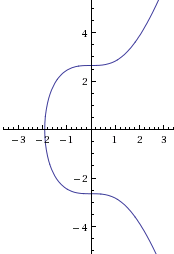
\includegraphics[width=0.30\textwidth]{introduction/secp256k1-graph}
	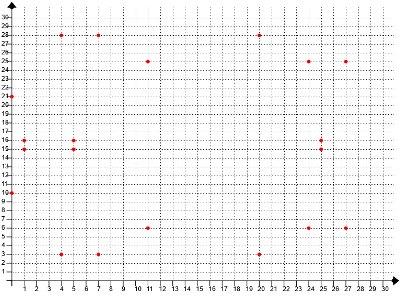
\includegraphics[width=0.59\textwidth]{introduction/secp256k1-graph-over-field-p31}
	\caption{The graph \(E: y^2 = x^3 + 0x + 7\) depicted left, and the same graph over the prime field
		\(\mathbb{F}_{31}\) depicted right. (Illustrated with http://www.wolframalpha.com \& http://www.graui.de)}
	\label{fig:graphs}
\end{figure}

ECC relies on the hardness of the elliptic curve discrete logarithm problem (ECDLP) to be secure. ECDLP is
defined as such: ``given an elliptic curve \(E\) defined over a finite field \(\mathbb{F}_q\), a point
\(P \in E(\mathbb{F}_q)\) of order \(n\), and a point \(Q \in \langle P \rangle\), find the integer
\(l \in [0,n-1]\) such that \(Q = lP\). The integer \(l\) is called the \emph{discrete logarithm of
\(Q\) to the base \(P\)}, denoted \(l = log_P Q\).''\footnote{The hardness of the adapted ElGamal (see
Section \ref{sec:math_encryption}) is exactly that of the ECDLP, with the public key \(Q\) and private
key \(l\).}\cite{hankerson2010}

\textbf{Note: Add something about patent problems (not many free implementations exist!) - which free
implementations do exist?}

\textbf{Note: Add paragraph on different types of curves (Weierstrass, Montgomery, Edwards).}

Elliptic curves provide a new mathematical model that can be used as the basis for cryptography,
as they allow for the creation of one-way "trapdoor" functions to be constructed.

In 1995, ElGamal described a simple (as in simply brilliant) public key cryptosystem that can be adapted
to use elliptic curves (Section \ref{sec:math_encryption_elgamal}). This system relies on the ability to
encode messages as points on an elliptic curve (Section \ref{sec:math_encoding}).

This paper describes the structure of \emph{OpenECC}, an open-source implementation of the functionality
described in the mathematical foundation section. \emph{OpenECC} has been developed concurrently with the
production of the paper, \textbf{(revise:) and is used as a basis for performance measurements, comparing the different constructs
with each other, measuring which are the most efficient (Section \ref{sec:performance}).}

The implementation is modular, allowing for different curves and encryption schemes to be swapped in and out
rapidly (Section \ref{sec:implementation}). As such, the library can be extended in the future to support different
curves, encodings, and encryption schemes. It also provides a readable syntax that makes it more easily
understandable than available alternatives, such as Bouncy Castle (Section \ref{sec:implementation_curves}).

While \emph{OpenECC} implements the constructs used specifically in elliptic curve cryptography it relies one external construct.
The elliptic curves rely on Bouncy Castle library's implementation of finite fields, which limits comparisons to the elliptic curve
layer (such comparisons are performed in Section \ref{sec:performance_bouncycastle}).

\textbf{Note: Add source to paragraph below! (NSA has something...)}

Comparisons of the security provided per key-length for different cryptographic algorithms exist.\footnote{Source?!} With
most mathematical operations - including those used in ECC - several performance optimizations exist over the naïve
implementation. The performance of traditional public-key cryptography implementations has been continuously improved
since its inception. To understand whether ECC is feasible as an alternative to traditional cryptography, the performance
of ECC must be evaluated in relation to that of traditional public-key cryptography implementations.

\textbf{Note: Something about SafeCurves here!}

\textbf{Note: There should be hints at the findings of the report here! (Performance...)}

\textbf{Note: Findings: Slow implementation --- but why? What are the points to improve?}

\textbf{Note: Focus on the potential for improvement...}

\textbf{Note: If BigInteger conversion is indeed what is slow, focus on the fact that a native finite field implementation would
solve many problems.}